\section{各画面の説明}
\subsection{ログイン画面}
\subsubsection{画面の概要}
% 画面の概要
この画面は、システムを利用する管理者および学生がログインするためのものです。
図\ref{fig:sc_login}にイメージ図を示します。

\begin{figure}[htbp]
  \begin{center}
    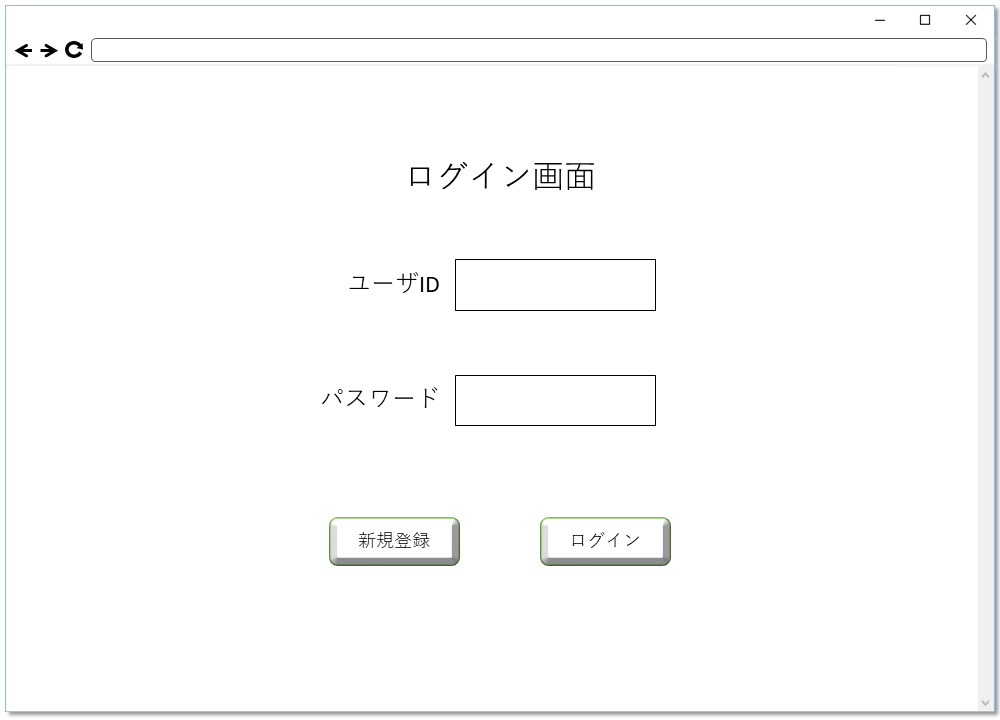
\includegraphics[width=1\linewidth,clip]{./img/sc_login.png}
    \caption{ログイン画面のイメージ図}\label{fig:sc_login}
  \end{center}
\end{figure}

\subsubsection{操作説明}
% 操作説明
アカウントを新規登録する場合は、
「新規作成」ボタンを押下すると、「アカウント新規作成画面」に遷移します。

ログインする場合は、
ユーザIDとパスワードを入力し、「ログイン」ボタンを押下します。
ログインが成功すると、管理者アカウントの場合は「授業選択画面」に遷移します。
学生アカウントの場合は「授業画面」に遷移します。
また、ログインが失敗すると、他の画面には遷移せず、もう一度ログイン画面が表示されます。

\subsection{アカウント新規作成画面}
\subsubsection{画面の概要}
% 画面の概要
この画面は、学生がアカウントを新規作成するためのものです。
図\ref{fig:sc_account_creat}にイメージ図を示します。

\begin{figure}[htbp]
  \begin{center}
    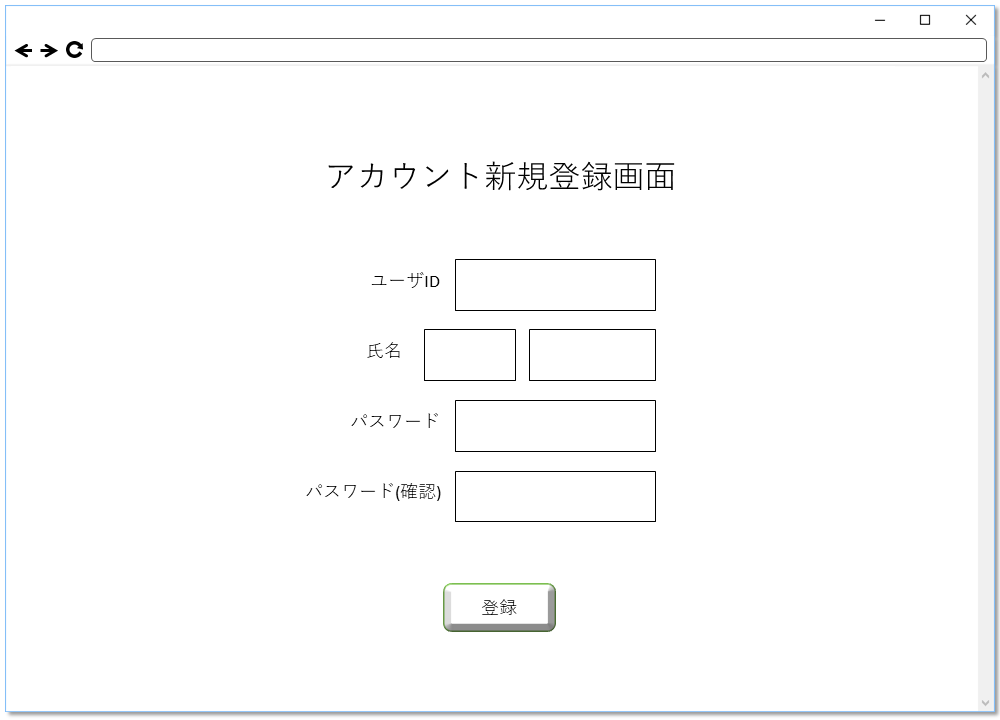
\includegraphics[width=1\linewidth,clip]{./img/sc_account_creat.png}
    \caption{アカウント新規作成画面のイメージ図}\label{fig:sc_account_creat}
  \end{center}
\end{figure}

\subsubsection{操作説明}
% 操作説明
ユーザID、氏名(フルネーム)およびパスワードを入力します。
なお、パスワードは確認のために2回入力します。
「登録」ボタンをクリックすると、「ログイン画面」に遷移します。

\subsection{管理者用の授業選択画面}
\subsubsection{画面の概要}
% 画面の概要
この画面は、管理者が担当する授業画面へのリンクが表示されています。
また、新規に授業画面を作成することもできます。
図\ref{fig:sc_select_class}にイメージ図を示します。

\begin{figure}[htbp]
  \begin{center}
    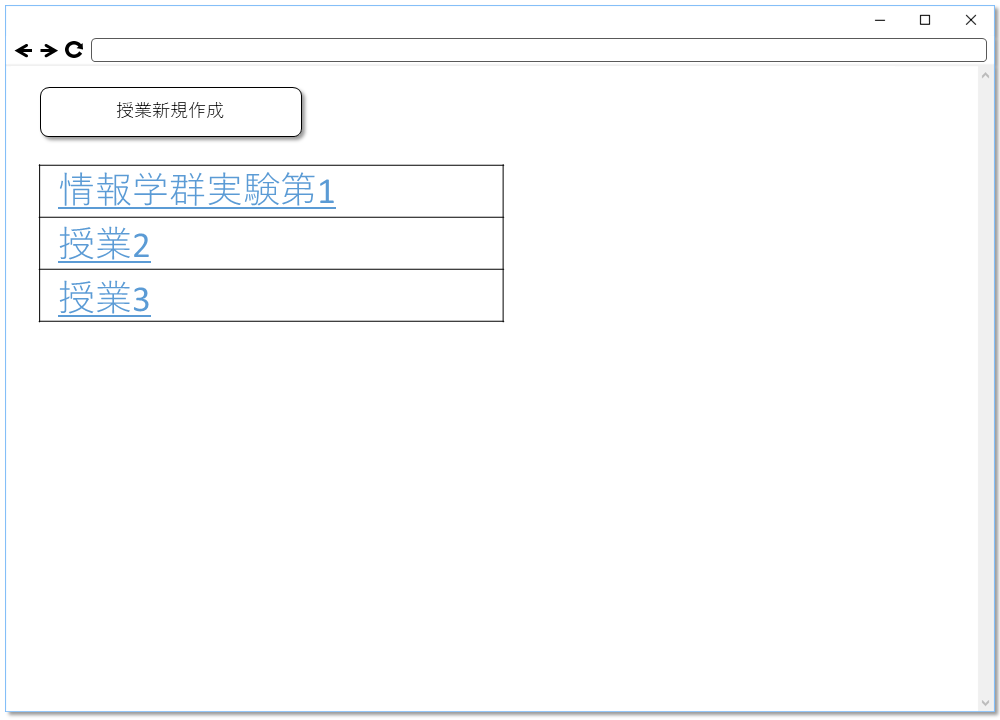
\includegraphics[width=1\linewidth,clip]{./img/sc_select_class.png}
    \caption{管理者用の授業選択画面のイメージ図}\label{fig:sc_select_class}
  \end{center}
\end{figure}

\subsubsection{操作説明}
% 操作説明
「授業新規作成」ボタンを押下すると、「授業カスタマイズ画面」に遷移します。
授業名がその授業画面へのリンクとして表示されているので、そのリンクを押下することで「管理者用の授業画面」に遷移します。

\subsection{授業新規作成画面}
\subsubsection{画面の概要}
% 画面の概要
この画面は、新しく授業を作成する時の、初期設定の画面です。
図\ref{fig:sc_select_class}にイメージ図を示します。

\begin{figure}[htbp]
  \begin{center}
    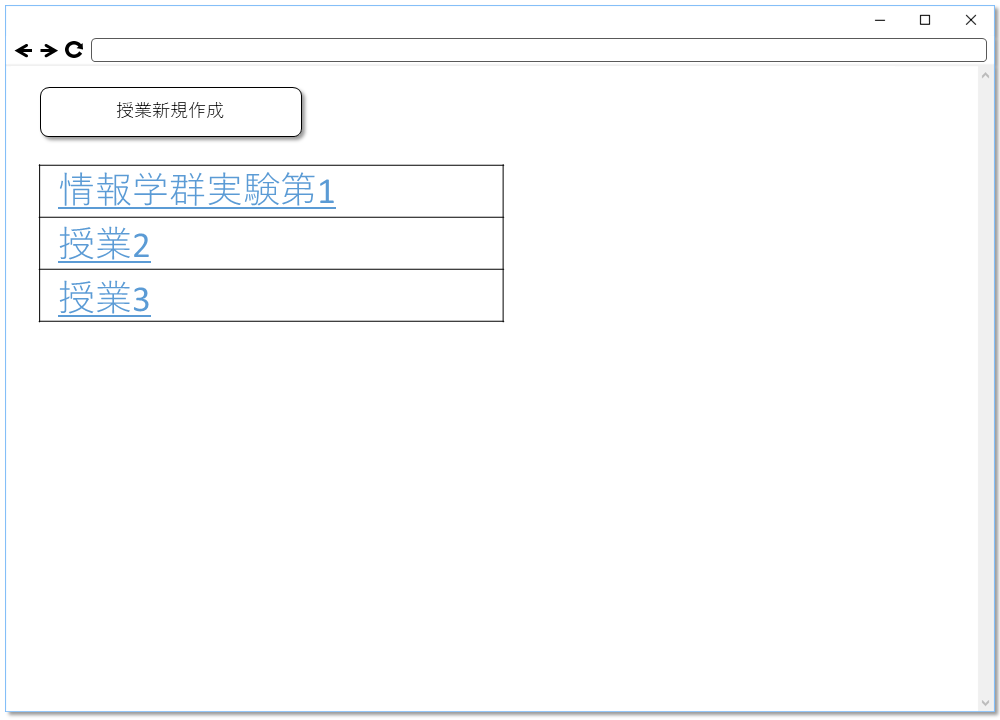
\includegraphics[width=1\linewidth,clip]{./img/sc_select_class.png}
    \caption{管理者用の授業選択画面のイメージ図}\label{fig:sc_select_class}
  \end{center}
\end{figure}

\subsubsection{操作説明}
% 操作説明
まず、授業名を授業名の欄に入力します。その後、この授業が何回行われるのかを授業回数の欄に入力します。
その後、グループワークなのか、個人ワークなのかによって、使用したいレイアウトをチェックボックスに選択し、決定ボタンを押すことで、詳細設定画面へと遷移します。

\subsection{授業詳細設定画1}
\subsubsection{画面の概要}
% 画面の概要
この画面は、「新規作成画面」で入力した授業回数に応じて、それぞれの回の授業タイトルと課題数を入力する画面です。
図\ref{fig:sc_class_detail1}、\ref{fig:sc_class_detail2}にイメージ図を示します。

\begin{figure}[htbp]
\begin{center}
  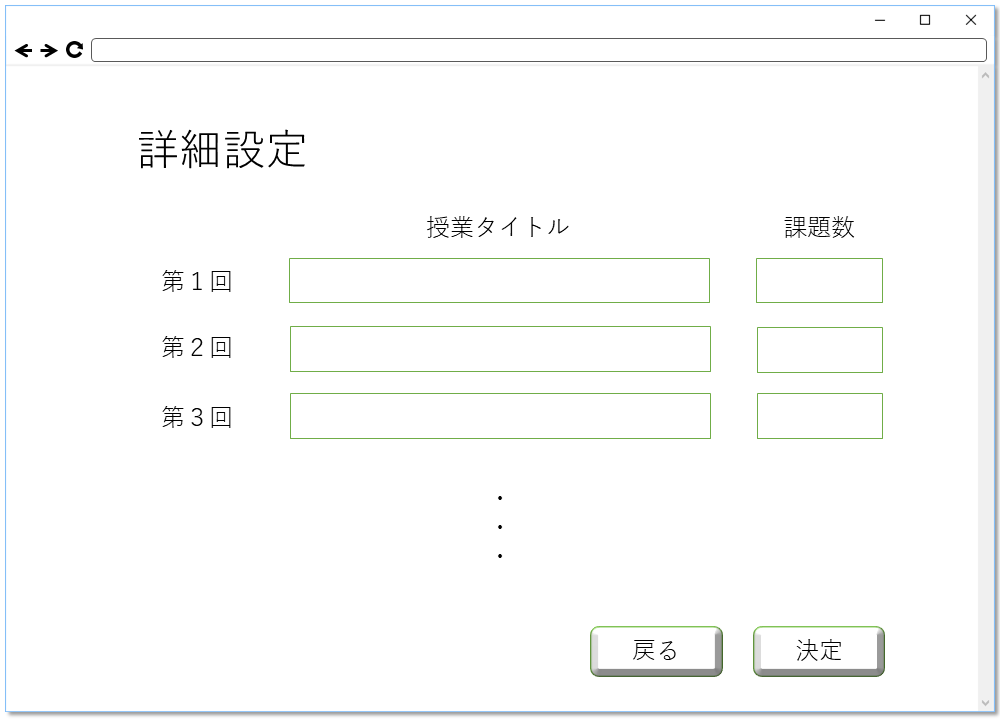
\includegraphics[width=1\linewidth,clip]{./img/sc_class_detail1.png}
  \caption{授業詳細設定画面のイメージ図1}\label{fig:sc_class_detail1}
\end{center}
\end{figure}

\subsubsection{操作説明}
% 操作説明
授業タイトルには学生側が過去の質問を見ようとした時でもわかるようなタイトルを入力
課題数にはその回に出る課題の数を入力
全て入力して終わったら決定ボタンで「詳細設定画面2」に移動する
戻るボタンで「新規作成画面」に戻る

\subsection{授業詳細設定画面2}
\subsubsection{画面の概要}
% 画面の概要
この画面は、この画面は「詳細設定画面1」で入力したタイトルとその課題数に応じて課題の内容を入力する画面に移動する前の画面です。
図\ref{fig:sc_class_detail1}、\ref{fig:sc_class_detail2}にイメージ図を示します。

\begin{figure}[htbp]
\begin{center}
  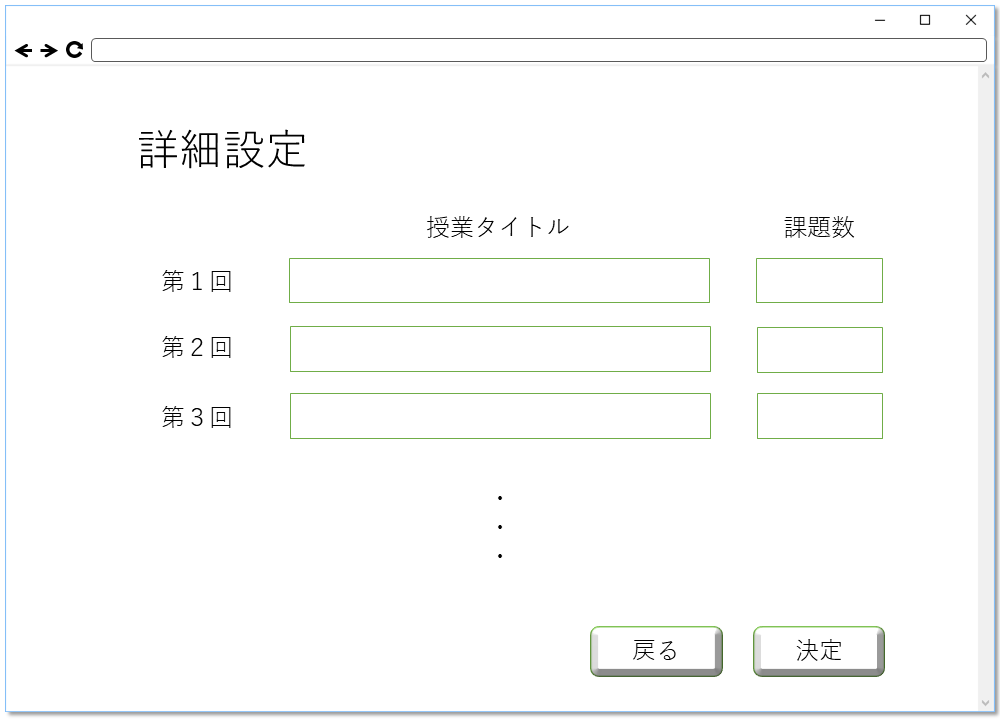
\includegraphics[width=1\linewidth,clip]{./img/sc_class_detail1.png}
  \caption{授業詳細設定画面のイメージ図1}\label{fig:sc_class_detail1}
\end{center}
\end{figure}

\subsubsection{操作説明}
% 操作説明
授業タイトルボタンを押すことでそのタイトルの課題内容を入力する「詳細設定画面3」に移動
全てのタイトルに応じた授業内容を入力し終わったら、決定ボタンを押すことで詳細設定を保存し、授業選択画面へと遷移します。

\subsection{授業詳細設定画面3}
\subsubsection{画面の概要}
% 画面の概要
この画面は、授業の各内容ごとに課題の詳細や、進捗確認画面で表示される課題名などを設定する画面です。
図\ref{fig:sc_class_detail1}、\ref{fig:sc_class_detail2}にイメージ図を示します。

\begin{figure}[htbp]
\begin{center}
  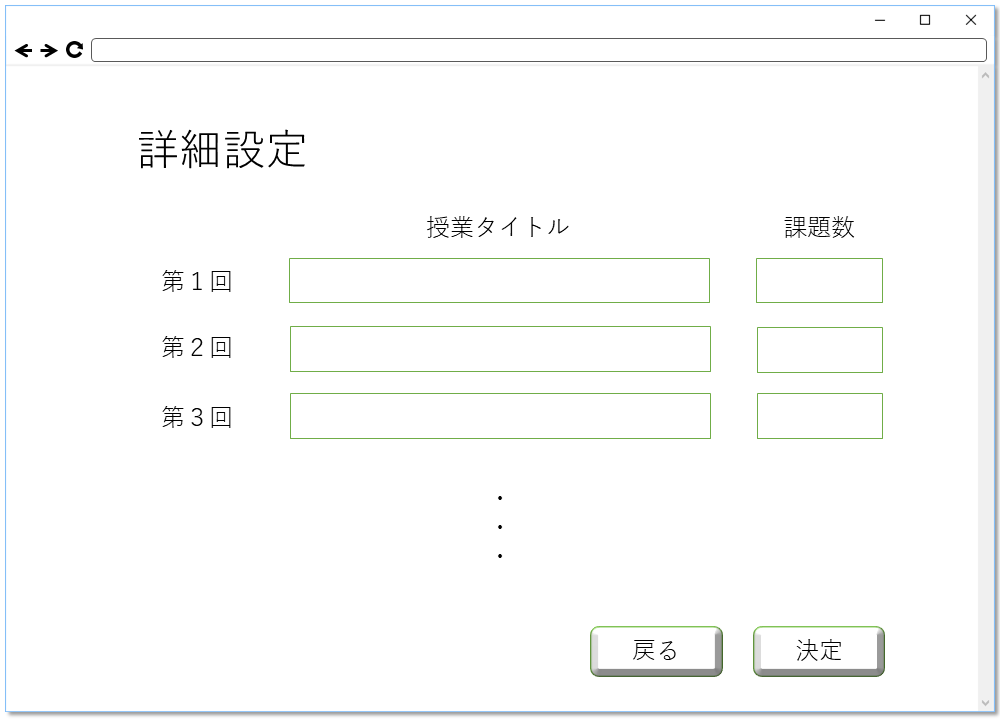
\includegraphics[width=1\linewidth,clip]{./img/sc_class_detail1.png}
  \caption{授業詳細設定画面のイメージ図1}\label{fig:sc_class_detail1}
\end{center}
\end{figure}

\subsubsection{操作説明}
% 操作説明
画面左側に詳細設定画面で入力した、課題数の数だけ課題内容を入力するテキストボックスが表示されます。
そのテキストボックス内に課題の内容を入力することで課題内容を設定できます。
画面右側には、進捗確認画面に表示される課題のタイトルを入力して行きます。
内容を入力したら、決定ボタンを押すことで内容が確定せれ、詳細設定画面2へと戻ります。

\subsection{管理者用の進捗確認画面(個人)}
\subsubsection{画面の概要}
% 画面の概要
この画面は、個人ワークに適したレイアウトの進捗確認画面になります。
図\ref{fig:sc_prog_check_one1}、\ref{fig:sc_prog_check_one2}にイメージ図を示します。

\begin{figure}[htbp]
\begin{center}
  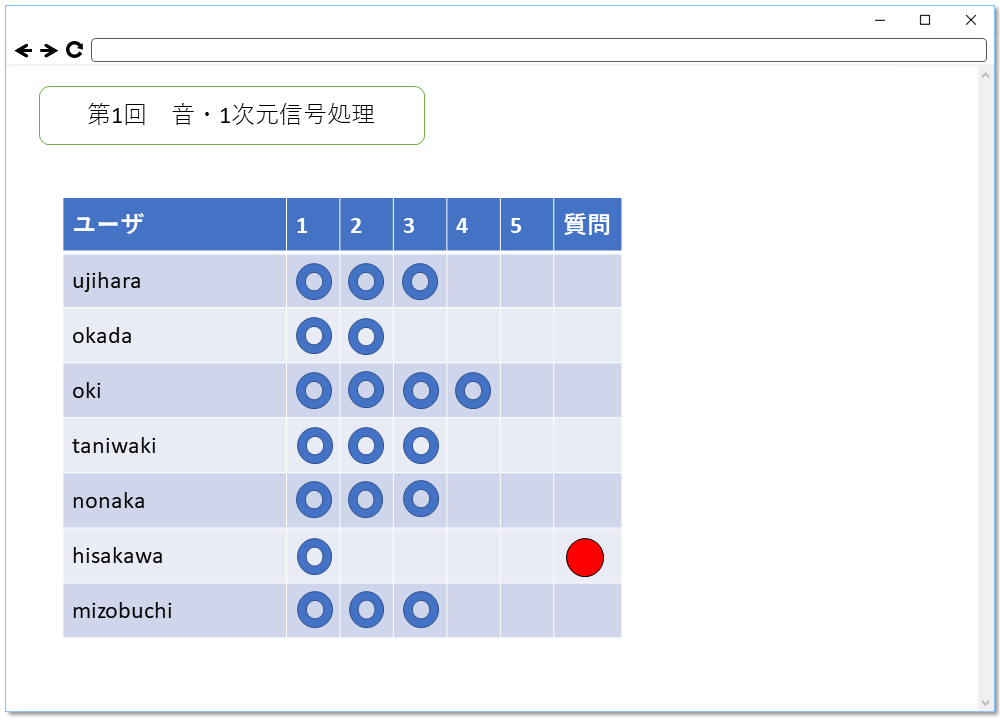
\includegraphics[width=1\linewidth,clip]{./img/sc_prog_check_one1.png}
  \caption{管理者用の進捗確認画面(個人)のイメージ図1}\label{fig:sc_prog_check_one1}
\end{center}
\end{figure}

\begin{figure}[htbp]
\begin{center}
  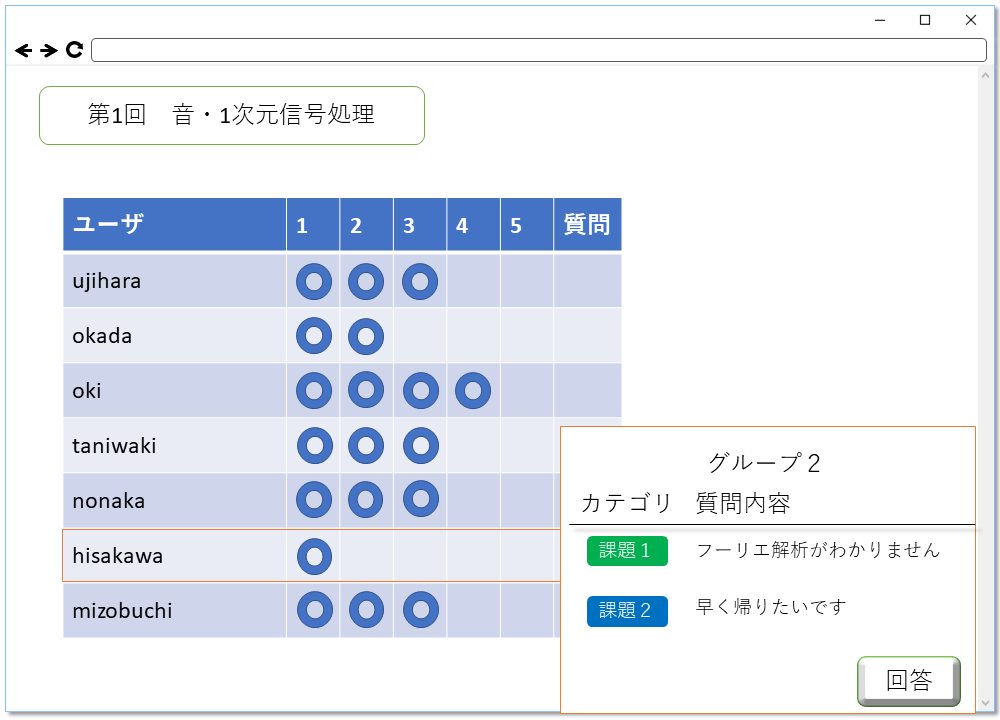
\includegraphics[width=1\linewidth,clip]{./img/sc_prog_check_one2.png}
  \caption{管理者用の進捗確認画面(個人)のイメージ図2}\label{fig:sc_prog_check_one2}
\end{center}
\end{figure}

\subsubsection{操作説明}
% 操作説明
表の形式でユーザごとの進捗が表示されており、ユーザ名の横に課題ごとの進捗が表示されて行きます。
また、学生から質問があると、その学生の一番右側の質問の欄が点灯します。
表内をクッリクすると、そのクリックしたユーザからの質問の確認が行えるウィンドウが開き、そのウィンドウの回答のボタンをクリックすることで、
質問回答画面へと遷移します。

\subsection{管理者用の回答画面}
\subsubsection{画面の概要}
% 画面の概要
この画面は、管理者が、学生から送信された質問に回答するためのものです。
図\ref{fig:sc_answer}にイメージ図を示します。

\begin{figure}[htbp]
\begin{center}
  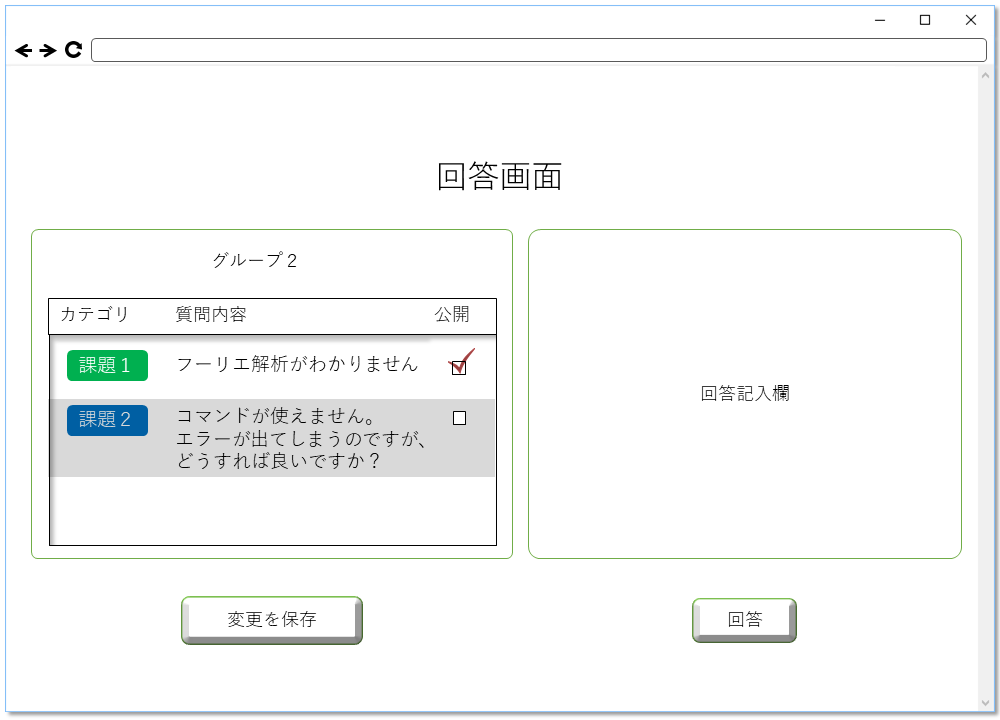
\includegraphics[width=1\linewidth,clip]{./img/sc_answer.png}
  \caption{管理者用の授業選択画面のイメージ図}\label{fig:sc_answer}
\end{center}
\end{figure}

\subsubsection{操作説明}
% 操作説明
質問回答画面には、左側にグループ名とそのグループからの質問が表示されています。
回答をする場合、その質問が表示されている部分を選択し、
右側にある回答記入欄に回答を記入し、回答ボタンをクリックすることで送信します。
質問や回答の内容は他の学生にも閲覧することが可能となっており、
その質問や回答の内容公開するかしないかは、
質問の横にある公開の欄にチェックすることで設定ができます。

\subsection{学生用ホーム画面}
\subsubsection{画面の概要}
% 画面の概要
この画面は、学生側のログイン後に表示される今年度の質問を確認したり、進捗状況を管理者側に送信したりできる、学生側にとってのホーム画面です。
画面上部に授業名が表示されており、その下に質問確認欄と進捗状況入力欄があります。
左側の質問確認欄には、受講中の内容に関する質問が表示されており、カテゴリ順に並べられています。
図\ref{fig:sc_class_student}にイメージ図を示します。

\begin{figure}[htbp]
\begin{center}
  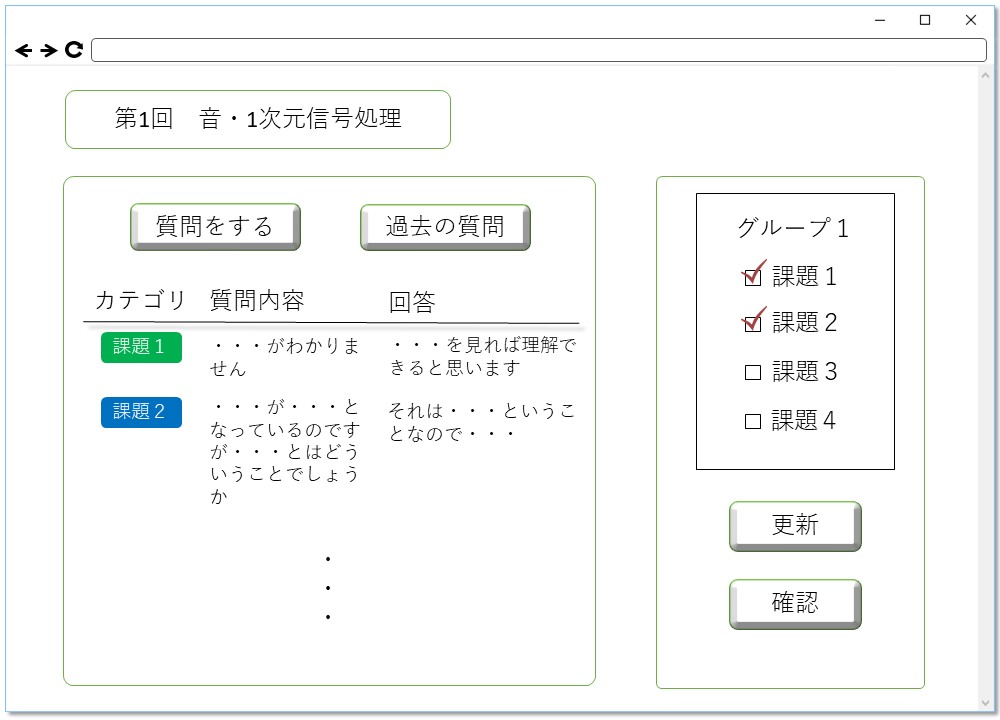
\includegraphics[width=1\linewidth,clip]{./img/sc_class_student.png}
  \caption{学生用ホーム画面のイメージ図}\label{fig:sc_class_student}
\end{center}
\end{figure}

\subsubsection{操作説明}
% 操作説明
過去の質問を確認する場合、質問確認欄にある「過去の質問」ボタンを押して年度選択画面に遷移します。
質問をする場合、質問確認欄にある「質問をする」ボタンを押して質問入力画面に遷移します。
進捗状況を管理者側に送信する場合、進捗状況入力欄にあるチェックボックスに終わった課題分チェックをつけて「更新」ボタンを押して更新を行います。
全ての課題を終えて管理者側に確認を行ってもらいたい場合、「確認」ボタンを押します。

\subsection{年度選択画面}
\subsubsection{画面の概要}
% 画面の概要
この画面は、学生側が過去の質問を確認する際にどの年度に出た質問を確認するのか選択する画面です。
図\ref{fig:sc_select_year}にイメージ図を示します。

\begin{figure}[htbp]
\begin{center}
  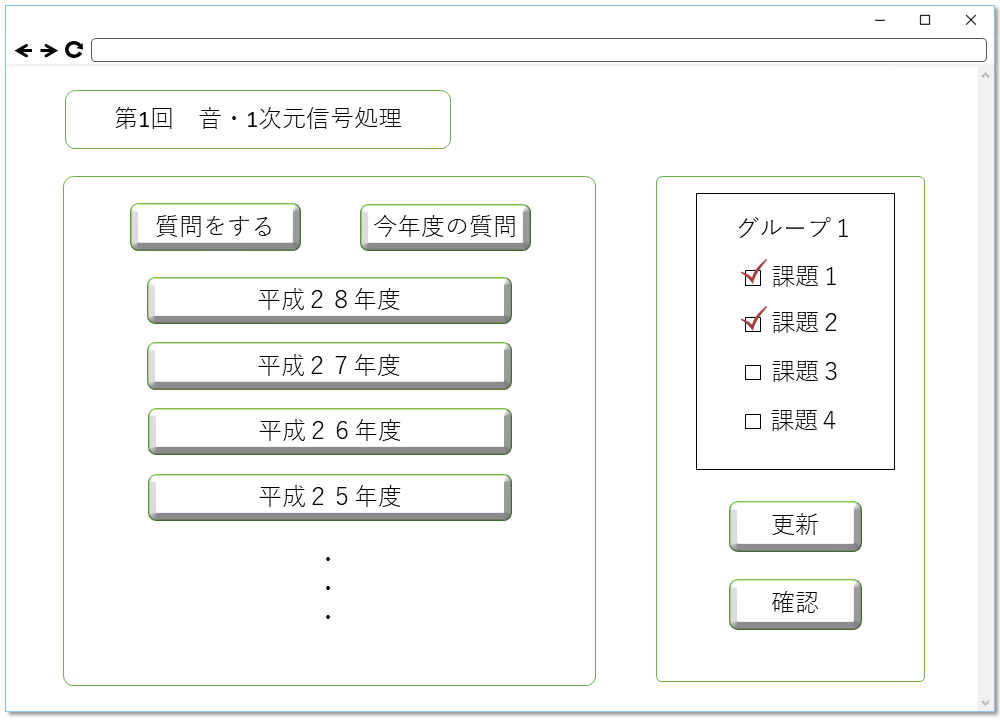
\includegraphics[width=1\linewidth,clip]{./img/sc_select_year.png}
  \caption{年度選択画面のイメージ図}\label{fig:sc_select_year}
\end{center}
\end{figure}

\subsubsection{操作説明}
% 操作説明
年度ボタンを押すと、その年度の「授業内容画面」に遷移します。
「今年度の質問」ボタンを押すと今年度の質問が表示されている「学生用ホーム画面」に戻ります。

\subsection{授業内容選択画面}
\subsubsection{画面の概要}
% 画面の概要
この画面は、学生側が選択した質問を確認したい年度に対する、授業の内容を選択する画面です。
図\ref{fig:sc_class_content}にイメージ図を示します。

\begin{figure}[htbp]
\begin{center}
  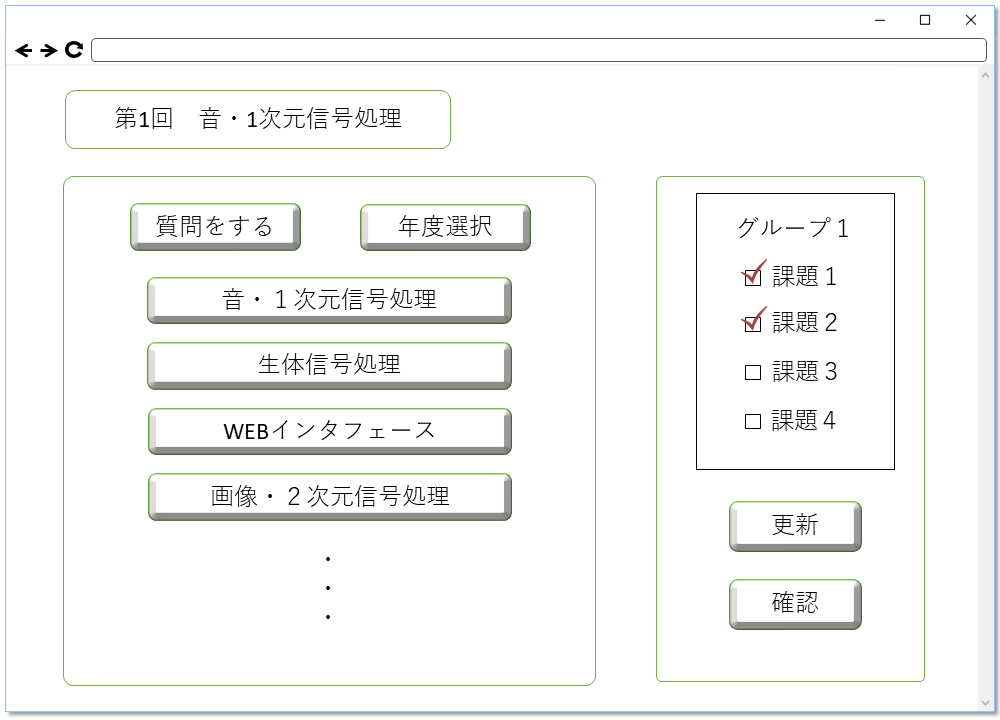
\includegraphics[width=1\linewidth,clip]{./img/sc_class_content.png}
  \caption{授業内容選択画面のイメージ図}\label{fig:sc_class_content}
\end{center}
\end{figure}

\subsubsection{操作説明}
% 操作説明
授業内容が書かれてあるタイトルを選択するとその回の授業で出た質問が表示される「過去質問画面」に遷移します。
「年度選択」ボタンを押すと「年度選択画面」に戻ります。

\subsection{過去質問画面}
\subsubsection{画面の概要}
% 画面の概要
この画面は、学生側が選択した条件に合わせて過去の質問が表示される画面です。
基本的な表示の仕方はホーム画面と同じです。
図\ref{fig:sc_pre_q}にイメージ図を示します。

\begin{figure}[htbp]
\begin{center}
  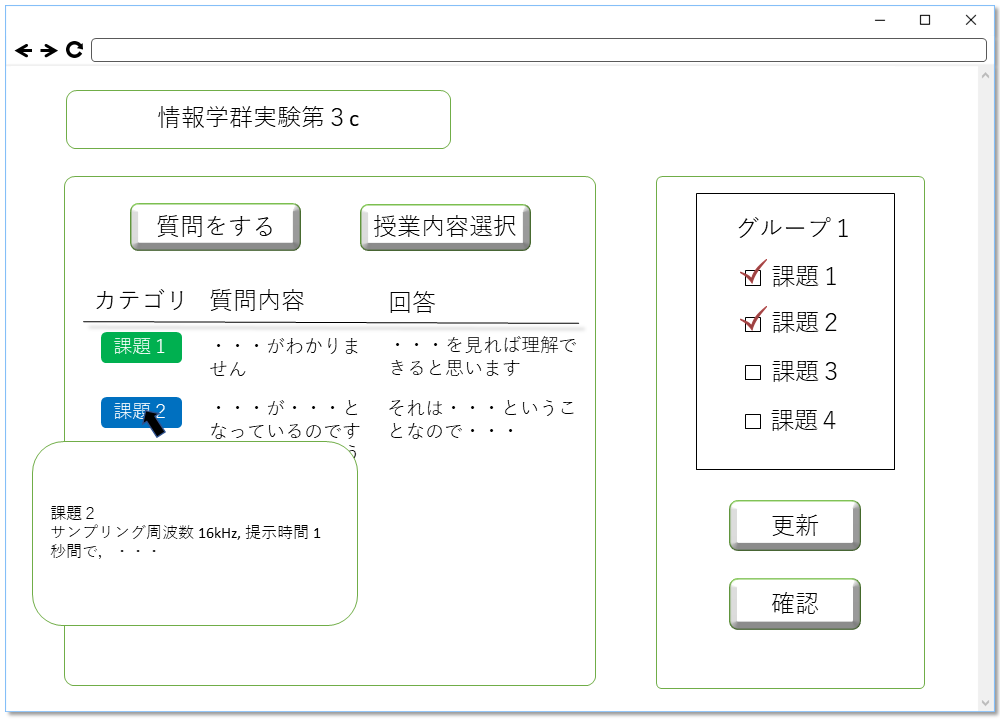
\includegraphics[width=1\linewidth,clip]{./img/sc_pre_q.png}
  \caption{過去質問画面のイメージ図}\label{fig:sc_pre_q}
\end{center}
\end{figure}

\subsubsection{操作説明}
% 操作説明
基本的には「学生用ホーム画面」と同じで違うところは、「授業内容選択」ボタンで「授業内容選択画面」に戻ることです。

\subsection{質問入力画面}
\subsubsection{画面の概要}
% 画面の概要
この画面は、学生側が管理者側に送信する質問内容を入力する画面です。
図\ref{fig:sc_input_q}にイメージ図を示します。

\begin{figure}[htbp]
\begin{center}
  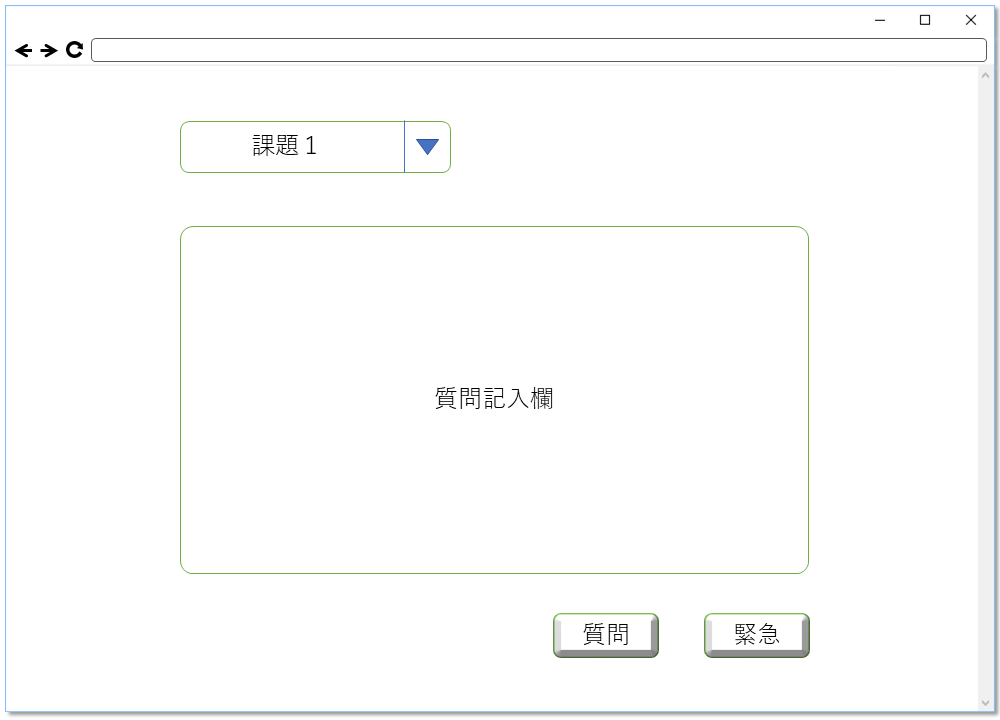
\includegraphics[width=1\linewidth,clip]{./img/sc_input_q.png}
  \caption{質問入力画面のイメージ図}\label{fig:sc_input_q}
\end{center}
\end{figure}

\subsubsection{操作説明}
% 操作説明
まず画面上部の三角を押して、どの課題に対して質問をするのか選びます。
次にその下の質問入力欄に質問内容を入力して、「質問」ボタンを押します。
PCに問題が起きた時などの緊急案件の場合は課題選択のところに用意してあるその他を選んでいただき、内容を書いて「緊急」ボタンを押していただきます。
2つのどのボタンを押しても管理者に内容を送信後、1つ手前の画面に戻ります。

\subsection{授業画面作成画面}
\subsubsection{画面の概要}
% 画面の概要
この画面は、。
図\ref{fig:sc_class_creat1}、\ref{fig:sc_class_creat2}にイメージ図を示します。

\begin{figure}[htbp]
\begin{center}
  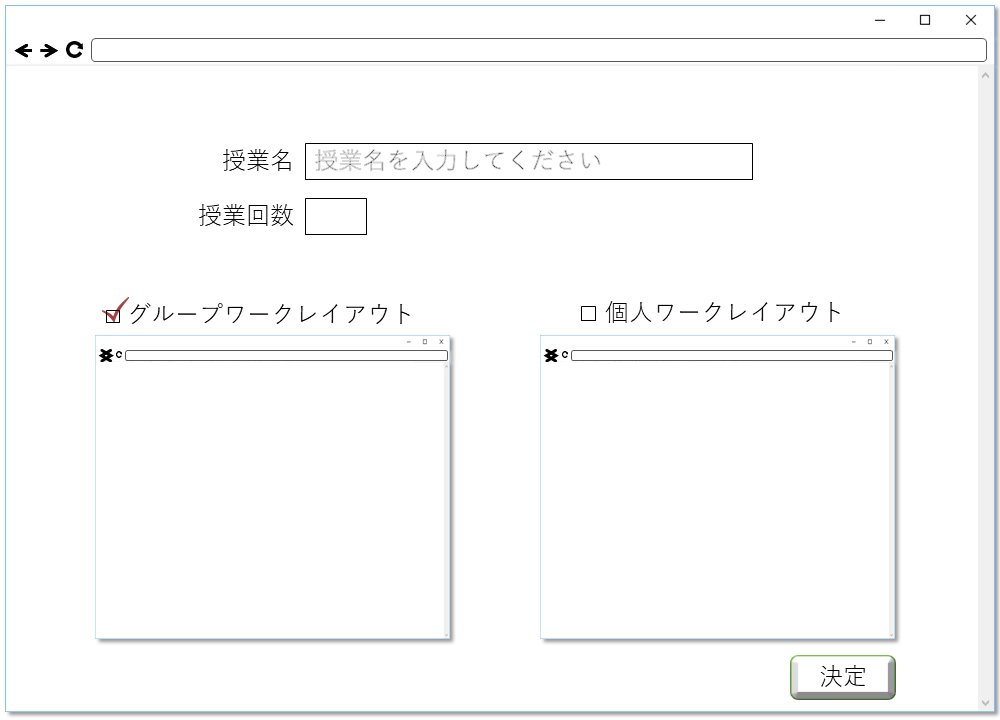
\includegraphics[width=1\linewidth,clip]{./img/sc_class_creat1.png}
  \caption{授業画面作成画面のイメージ図1}\label{fig:sc_class_creat1}
\end{center}
\end{figure}

\begin{figure}[htbp]
\begin{center}
  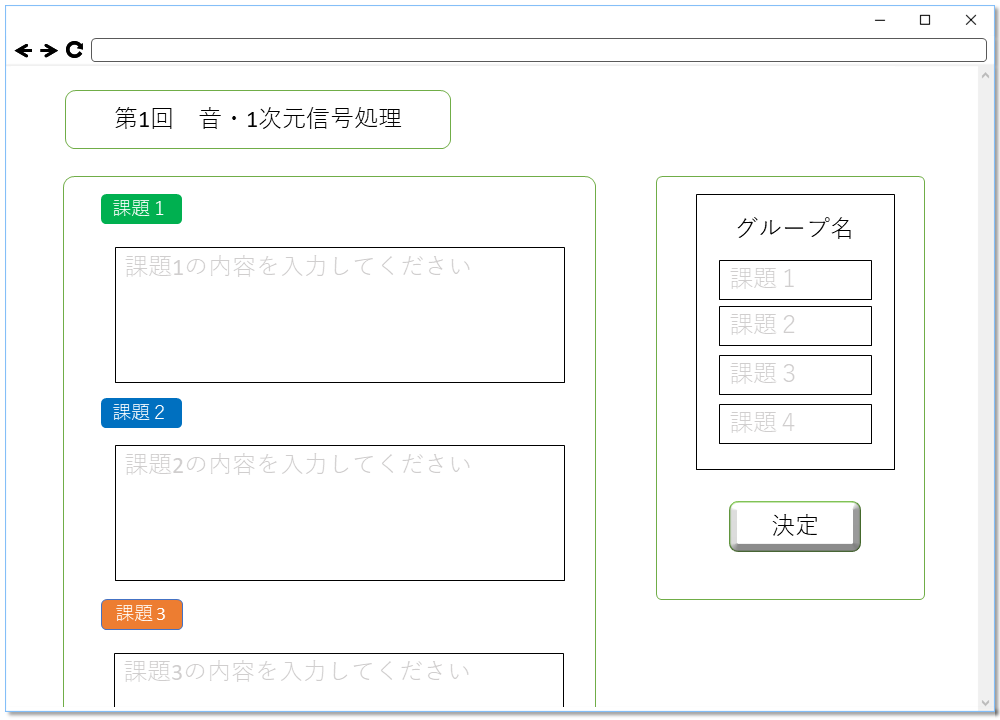
\includegraphics[width=1\linewidth,clip]{./img/sc_class_creat2.png}
  \caption{授業画面作成画面のイメージ図2}\label{fig:sc_class_creat2}
\end{center}
\end{figure}
